\documentclass{article} % For LaTeX2e
\usepackage{nips13submit_e,times}
\usepackage{amsmath}
\usepackage{amssymb}
\usepackage{comment}
\usepackage{hyperref}
\usepackage{enumerate}
\usepackage{enumitem}
\usepackage{cleveref}
\usepackage{graphicx}
\usepackage{url}
\usepackage{placeins}
\usepackage{fancyvrb}
\usepackage[font={small,it},width=5in]{caption}
%\documentstyle[nips13submit_09,times,art10]{article} % For LaTeX 2.09


\title{Musical Structure in Irish Traditional Tunes}

\author{Matthew Staib, Lennart Jansson, and Edward Dai}

\newcommand{\fix}{\marginpar{FIX}}
\newcommand{\new}{\marginpar{NEW}}

\newcommand{\xip}{x^{(i)}}
\newcommand{\xjp}{x^{(j)}}
\newcommand{\xkp}{x^{(k)}}
\newcommand{\yip}{y^{(i)}}
\newcommand{\yjp}{y^{(j)}}
\newcommand{\ykp}{y^{(k)}}
\newcommand{\vectornorm}[1]{\left\| #1 \right\|}

\nipsfinalcopy % Uncomment for camera-ready version

\begin{document}

\maketitle

\section{Introduction}
Most Irish traditional folk dance music contains two musical themes; the tune
begins with one musical theme which is usually repeated, then progresses to
another theme with similar musical structure and motives, which is usually also
repeated. The first section is typically called the $A$ section while the second
is called the $B$ section. Our goal is to understand, at a quantitative level,
the relationship between $A$ sections and $B$ sections.

In working towards this goal, we need to understand both the relationship
between the $A$ and $B$ sections of a given folk song as well as the differences
between $A$ and $B$ sections of such music in general. In the long term we wish
to, given an $A$ section, automatically generate a musically appropriate $B$
section.

\section{Dataset}

We are using the tunes dataset from The Session \cite{thesession}. The
Session is an online community of people who are interested in playing Irish
folk music and cataloguing traditional Irish tunes for others to learn. These
tunes include various dance forms, such as jigs, reels, waltzes, and slides.
Available on their website is a set of roughly 21,000 dance tune settings
in ABC notation, a human-readable symbolic music data format in plain text. The
ABC files are easily parsed and manipulated symbolically for feature extraction.

\section{Feature Extraction}

First we select from our dataset tunes which have an $A$ and a $B$ section. We
consider only tunes with a number of bars in $\{16, 32, 64\}$: an individual $A$
or $B$ section usually has 8 or 16 measures, or 16 or 32 after unrolling repeat
signs. We want to restrict to tunes that split evenly into two sections (e.g.
not three sections, which could mean $ABC$, $ABA$, etc.).

After splitting tunes into $A$ and $B$ sections, we turn our attention to
feature extraction.  Our dataset is loosely in the form of sequences of pitches
representing melodies. However, as tunes may have different lengths, we need to
generate a feature vector of fixed length.

We define an $n$-gram as an ordered list of (in our case) $n$ pitches of notes
in a melody, ignoring accidentals. In total, we created three different feature
vectors.
\begin{enumerate}
%TODO: consider using nouns instead of verbs.
\item Record counts of all 1- and 2-grams.

\item Split melodies by measure into eighths and store counts of all 1- and
2-grams separately for each measure.

\item Use the features from (2), also adding counts of notes of each length.
\end{enumerate}

Since these feature vectors have nearly 2,000 components, before further
processing, we used PCA to reduce the number of components. This helped us
understand, to some extent, the bias caused by overfitting (as we will see
later), as well as made metric learning computationally more feasible.

\section{SVM Classifier}
Using our labeled pool of $A$ and $B$ sections, we used an SVM with Gaussian
kernel to attempt to classify a given segment of a tune as an $A$ section or a
$B$ section. We used 8-fold cross-validation, and experimented with our three
different feature vectors and various numbers of PCA components.

%TODO: (Lennart) Check the graph (re-run). You are responsible for updating this
%section of the paper.

\begin{figure}
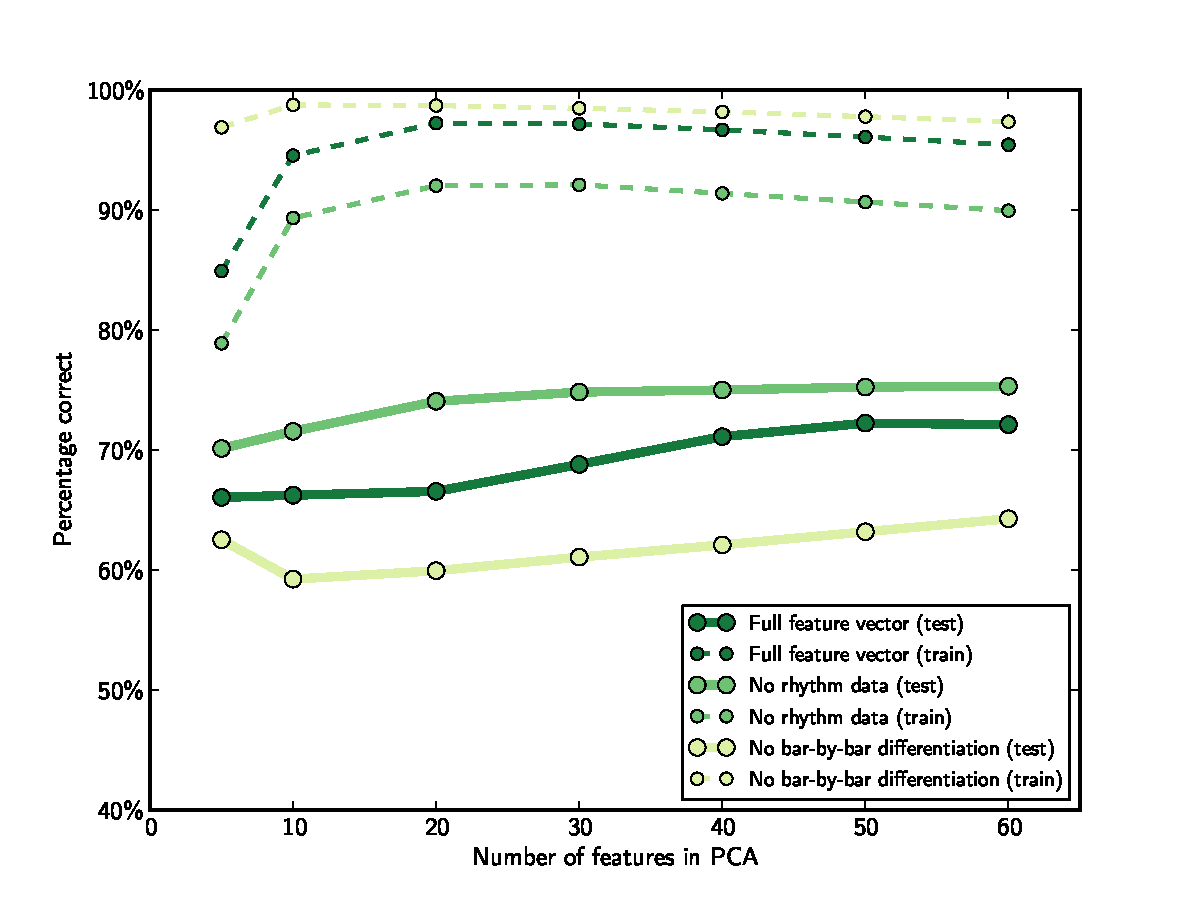
\includegraphics[width=5in]{../svm_results/svm.pdf}
%TODO: Add caption
%TODO: Add labels
\end{figure}

Observe that when we use the more complex feature vectors, training performance
improves, but test performance suffers. We attribute this to overfitting;
namely, as our feature vectors become more descriptive, the SVM identifies
particular patterns present only in the training data.

\section{Metric Learning Problem Formulation}
We also want to learn what makes the $A$ and $B$ sections of a particular tune
musically related. We attempt to learn a metric $d(x, y)$ where, if $x, y \in
\mathbb{R}^n$ are the feature vectors corresponding to the $A$ and $B$ sections
of a tune, $d(x, y)$ should be small. For this task, we use the Mahalanobis
metric, given by
\[
d(x,y) = \vectornorm{x-y}_M = \sqrt{(x-y)^T M (x-y)}
\] 
for $M \in \mathbb{R}^{n\times n}$ positive semidefinite, and attempt to learn a
suitable value of $M$.

Usually, in metric learning, one learns a metric by supplying both pairs of
points $(\xip, \xjp) \in \mathcal{S}$ that are similar and should have small
distance, and points $(\yip, \yjp) \in \mathcal{D}$ that are dissimilar and
should have large distance. We then solve the following optimization problem for
$M$: %TODO: Citation
\begin{align*} 
\text{minimize: } &
\sum_{(x^{(i)}, x^{(j)}) \in \mathcal S} \vectornorm{x^{(i)} - x^{(j)}}_M^2 \\
\text{subject to: }
& \sum_{(y^{(i)}, y^{(j)}) \in \mathcal D}
	\vectornorm{y^{(i)} - y^{(j)}}_M^2 \ge 1,
\quad\quad\quad\quad\quad\quad \cite{metricNg} \\
& M \succeq 0.
\end{align*} 
However, in our problem, it is unclear how to select pairs of $A$ and $B$
sections that are dissimilar. Intuitively, one might argue that the $A$ and $B$
sections of different tunes should be dissimilar. However, two arbitrary tunes
may be variations of each other, and hence have $A$ and $B$ sections that are
related.

Note that by simply removing the dissimilarity constraint results in an
optimization problem whose optimal value $M$ is the zero matrix. Instead, we
enforce $\det M = 1$ as a reasonable-seeming regularity constraint. We do this
by noting that $(\det M)^{1/n}$ is concave and so $(\det M)^{1/n} \ge 1$ is a
convex constraint. Then, the optimization problem,

\begin{align*} 
\text{minimize: } & \sum_{k=1}^m \vectornorm{x^{(k)} - y^{(k)}}_M^2 \\
\text{subject to: }
& M \succeq 0, \\
& (\det M)^{1/n} \ge 1,
\end{align*} 
where $m$ is the number of training examples, produces $M$ with $\det M = 1$, as
the objective function scales with the determinant of $M$.

\section{Metric Learning Results}

After using PCA to reduce our feature vectors to $n = 35$ components, we applied
this method using 8-fold cross-validation to learn such a metric $d$. To
evaluate the success of our metric, we consider the following problem:
\begin{itemize}
\item[] Split apart the $A$ and $B$ sections of our test data ($\approx 1000$
tunes). For each $A$ section, order all the $B$ sections by increasing distance
from this $A$ section (under the metric $d$). Record the rank in this list of
the actual corresponding $B$ section. Ideally, the actual $B$ section would be
the first element of this list, closest to this $A$ section. Alternatively, we
could match an $A$ section to a given $B$ section.
\end{itemize}
We made a cumulative histogram of the ranks of the actual sections.%TODO: See Figure
We also broke down the frequency of these ranks into a pie chart. %TODO: Fig
If we were to randomly guess the closest $B$ section, we would expect the rank
of the correct $B$ section to be 1 with probability 0.1\%. In our results, the
correct $B$ section was the first ranking option 37\% of the time. Moreover, the
correct $B$ section was in the top 10\% of the ranking 93\% of the time. We
conclude that there is a significant amount of information shared between $A$
sections and $B$ sections.
%TODO: caption and labels and resize
\begin{figure}
\begin{center}
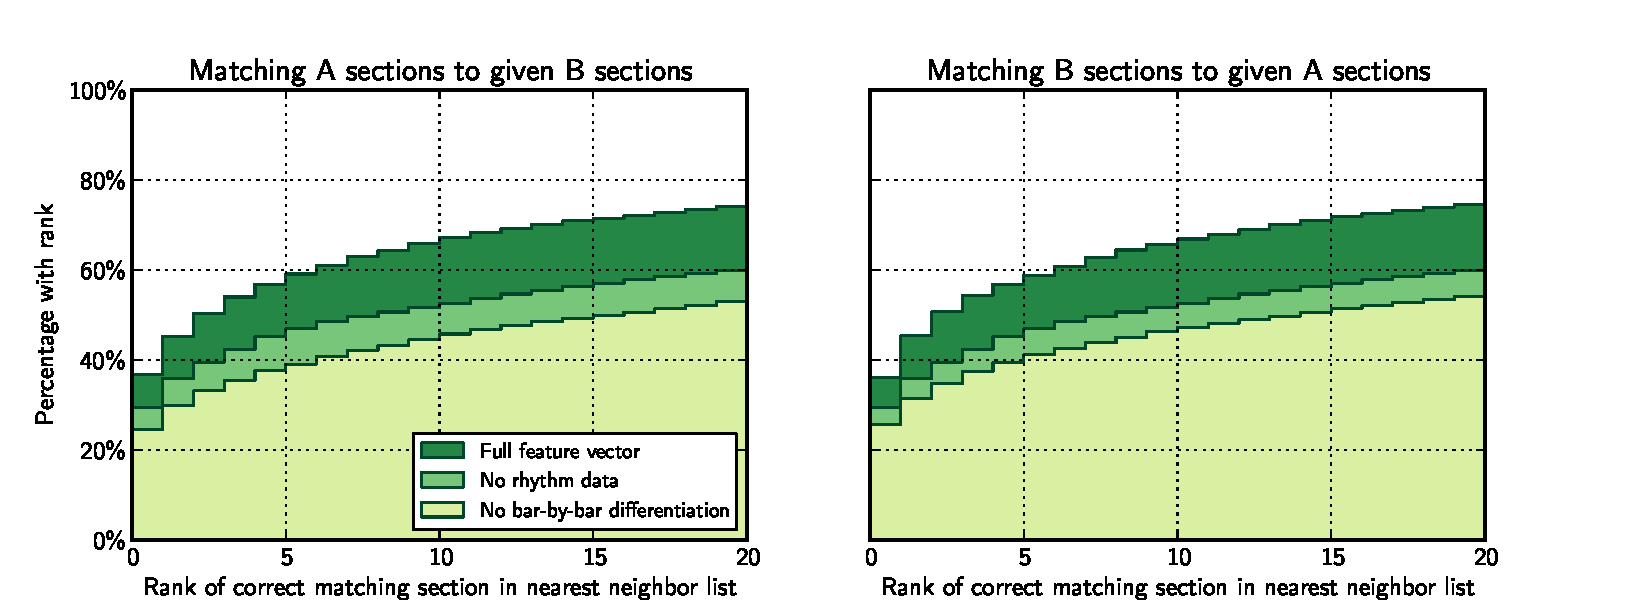
\includegraphics[width=2.5in]{../trial_data_logs/hists.pdf}
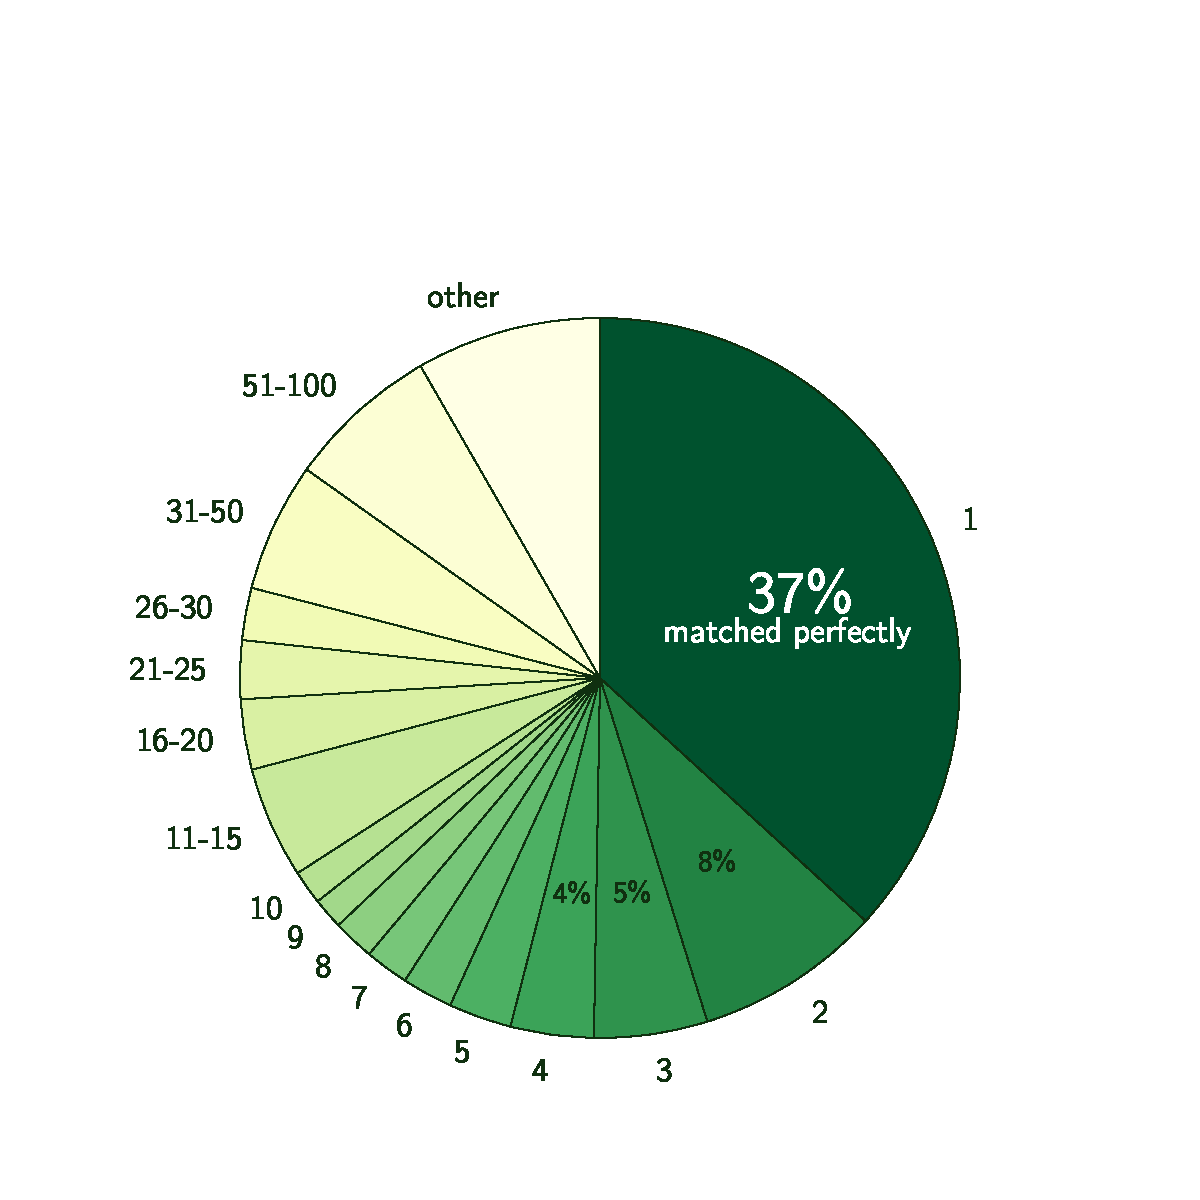
\includegraphics[width=2.5in]{../trial_data_logs/pie.pdf}
\end{center}
\end{figure}

\section{Composition}
Now that we have shown the viability of our metric, we can use it to try to,
given an $A$ section, compose a musically related $B$ section. We employed a
simple algorithm:
\begin{enumerate}
\item Select a specific tune, and split it into its $A$ and $B$ sections.

\item Randomize a $B$ section ($b_{cur}$) using the rhythm of the $A$ section.

\item Repeat $n$ times:
\begin{itemize}\parskip=0.05in
\item[] For every $i \in \{1, \dots, k\}$:
\begin{itemize}
\item[] Generate $b_i$ by randomly making pitch edits to $b_{cur}$.
\end{itemize}
\item[] Set
$\displaystyle{b_{cur} := \arg \min_{b_i} \  d(b_i, A)}$.
\end{itemize}
\end{enumerate}
As an example, we tried to compose a new $B$ section for the $A$ section of the
tune Cooley's Reel. %TODO (Lennart) Add music and figure.

While the resulting $B$ section is musically far from ideal, it is notably
better than the random starting $B$ section. For example, the starting note is
the same as that of the tune and the intervals between consecutive notes are, on
average, smaller.

\section{Further Work}
%TODO: Lennart



%I gave up. We're using this instead of the BibTex database. (ED)
%Format is "\bibitem{cite_key} bibliographic information ...."
%Cite using \cite{cite_key}.
\begin{thebibliography}{9}

\bibitem{thesession} 
The Session (\texttt{thesession.org}).

\bibitem{metricNg} 
E. Xing, A. Ng, M. Jordan, and S. Russell. Distance Metric Learning, with
Application to Clustering with Side-Information. \textit{NIPS}. 2002.

%TODO: Finish the references
%
%\item CVX
%
%\item Scikit Learn
%
%\item Boyd's Course Notes
%
%\item CVX User Guide
\end{thebibliography}

\end{document}
